\subsection{Single-process system call overheads}
\label{eval:perf:syscalls}


In order to understand the overheads of individual system calls,
Table~\ref{tab:eval:lmbench-syscalls} lists 
a representative sample of 
tests from the
\lmbench{} suite, version 2.5~\cite{McVoy:lmbench}.
Each row reports a mean and 95\% confidence interval;
we use the default number of iterations for each test case.
%We have added code to \lmbench{} to also calculate 95\% confidence intervals 
%within a run~\footnote{The lmbench authors deliberately exclude variation statistics
%because most methods assume a known distribution, generally a normal distribution---an 
%assumption which is often not the case for a computer microbenchmark~\cite{staelin05lmbench}.
%Though confidence intervals should be taken with a grain of salt, 
%we include them because they clearly indicate that these experiments have very low variance. In 
%a few cases of minor performance improvement, one can assess the impact of noise.}.
To measure the marginal cost of the reference monitor, we report numbers with and without 
the reference monitor.

%The performance of \graphene{} relative to Linux varies
%based on the system call.  
In general, calls that can be serviced inside the library are faster than native,
whereas calls that require translation to a native call incur overheads typically under 100\%.
For instance, 
the self-signaling test (sig overhead)
just calls the signal handler as a function,
which is almost twice as fast
as the Linux kernel implementation.  

\begin{table}[htp!]
\footnotesize
\centering
\bgroup
\def\arraystretch{1.1}
\setlength{\tabcolsep}{.5em}
\begin{tabular}{|ll|>{\palign{r}}p{3em}r|>{\palign{r}}p{3em}rr|>{\palign{r}}p{3em}rr|>{\palign{r}}p{3em}rr|}
\hline
& & \multicolumn{11}{c|}{System call latency (\usec{}), +/- Confidence Interval, \% Overhead} \\
\hline
\multicolumn{2}{|c|}{{\bf Test}} &
\multicolumn{2}{c|}{{\bf Linux \linuxversion{}}} &
\multicolumn{3}{c|}{{\bf \graphene{}}} & \multicolumn{3}{c|}{{\bf \graphene{}+SC+RM}} & \multicolumn{3}{c|}{{\bf \graphenesgx{}}} \\
& &
\usec{} & +/- & 
\usec{} & +/- & \%O &
\usec{} & +/- & \%O &
\usec{} & +/- & \%O \\
\hline																					
\multicolumn{2}{|l|}{{\tt getppid}}			&	0.045	&	.000	&	0.015	&	.000	&	-67	&	0.015	&	.000	&	-67	&	0.015	&	.000	&	-67		 \\\hline
\multicolumn{2}{|l|}{{\tt getppid} (direct)}			&	0.045	&	.000	&	\multicolumn{3}{c|}{Not supported}					&	1.155	&	.000	&	2,467	&	5.800	&	.001	&	12,789		 \\\hline
\hline																										
{\tt open}	&	{\tt /dev/zero}	&	0.997	&	.072	&	1.247	&	.000	&	25	&	1.256	&	.000	&	26	&	1.207	&	.004	&	21		 \\\hline
{\tt stat}	&	{\tt /dev/zero}	&	0.362	&	.000	&	0.466	&	.000	&	29	&	0.467	&	.000	&	29	&	0.451	&	.000	&	25		 \\\hline
{\tt fstat}	&	{\tt /dev/zero}	&	0.117	&	.000	&	0.111	&	.000	&	-5	&	0.111	&	.000	&	-5	&	0.107	&	.000	&	-9		 \\\hline
{\tt read}	&	{\tt /dev/zero}	&	0.116	&	.000	&	0.121	&	.000	&	4	&	0.121	&	.000	&	4	&	0.115	&	.000	&	-1		 \\\hline
{\tt write}	&	{\tt /dev/zero}	&	0.077	&	.000	&	0.116	&	.000	&	51	&	0.116	&	.000	&	51	&	0.112	&	.000	&	45		 \\\hline
\hline																										
install	&	sigaction	&	0.146	&	.000	&	0.113	&	.000	&	-23	&	0.113	&	.000	&	-23	&	0.110	&	.000	&	-25		 \\\hline
send	&	{\tt SIGUSR1}	&	0.895	&	.000	&	0.189	&	.000	&	-79	&	0.187	&	.000	&	-79	&	0.178	&	.000	&	-80		 \\\hline
catch	&	{\tt SIGSEGV}	&	0.379	&	.000	&	1.526	&	.000	&	303	&	1.575	&	.000	&	316	&	6.117	&	.000	&	1,514		 \\\hline

\end{tabular}
\egroup
\caption{System call benchmark results based on \lmbench{} 2.5. Comparison is among (1) native Linux processes, (2) \graphene{} \picoprocs{} on Linux host, both without and with JIT-optimized SECCOMP filter ({\bf +SC}) and reference monitor ({\bf +RM}), and (3) \graphene{} in SGX enclaves.
System call latency is in microseconds, and lower is better.
System call bandwidth and throughput are in megabytes per second and operations per second, respectively, and higher is better. 
%The file system is measured in thousands operations per second, and higher is better.
Overheads are relative to Linux \linuxversion{}; negative overheads indicate improved performance.} 
\label{tab:eval:lmbench-syscalls}
\end{table}








%\begin{figure*}[t!]
%\centering
%\footnotesize
%\begin{minipage}{.49\linewidth}
%\centering
%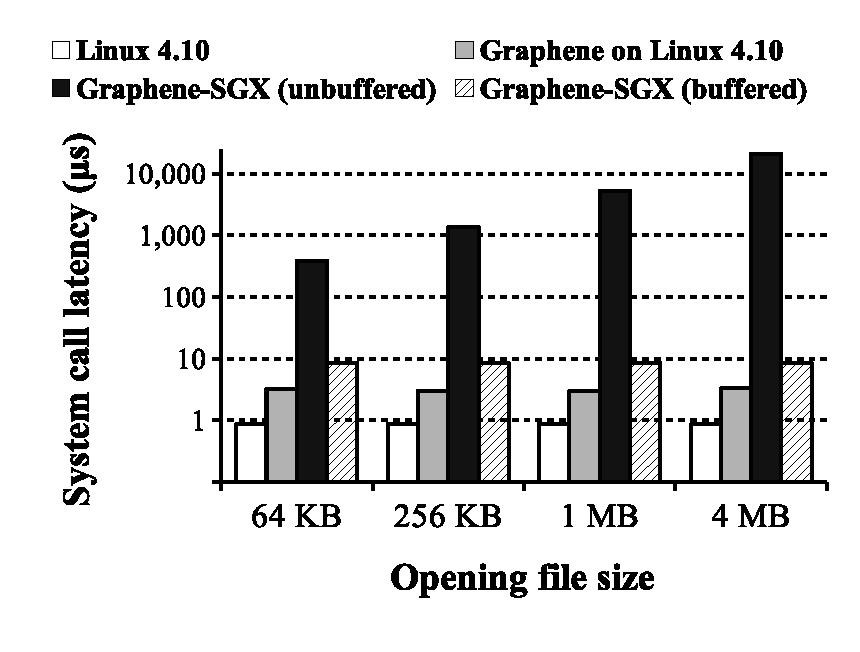
\includegraphics[width=24em]{open-latency}\\
%{\bf (a) Opening a file}
%\vspace{6pt}
%\end{minipage}
%\begin{minipage}{.49\linewidth}
%\centering
%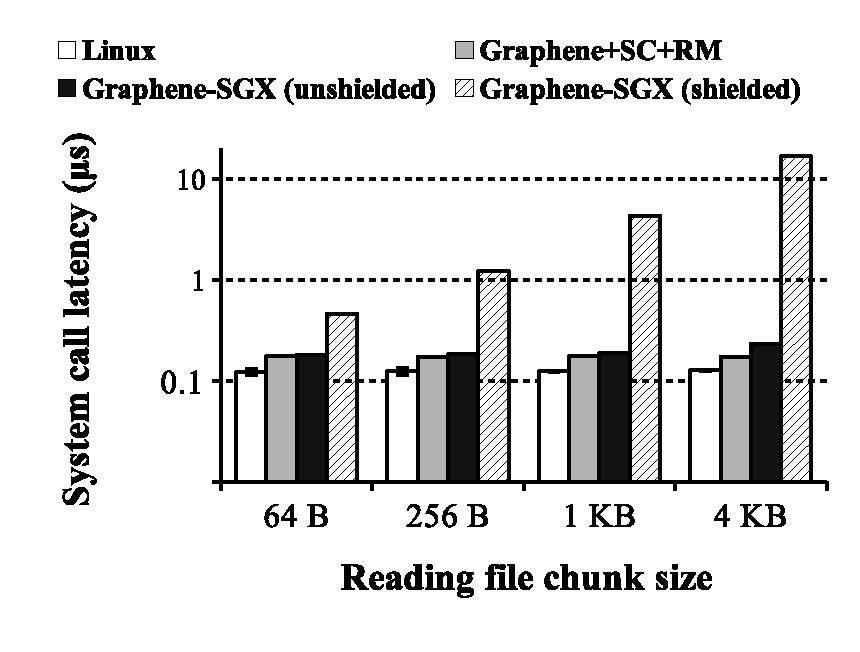
\includegraphics[width=24em]{read-latency}\\
%{\bf (b) Reading a file}
%\vspace{6pt}
%\end{minipage}
%\caption{Latency of some expensive system calls in \graphenesgx{}, including opening and reading a secured (authenticated) file, and forking a new process. The results are compared with native Linux and \graphene{}.}
%\label{fig:eval:sgx-open-read}
%\end{figure*}


%Figure~\ref{fig:eval:sgx-open-read}(a)
%shows the overhead for authenticating files in \syscall{open}.
%\fixme{change overhead to latency}
%Depending on the file size, the latency of \syscall{open} on \graphenesgx{} is 383$\mu$s (64KB file) to 21ms (4MB file), whereas on Linux, the latency is constant at 0.85$\mu$s.
%We note that this is where enclaves are at a disadvantage, as \syscall{open} 
%normally does not need to read file content; whereas here \graphenesgx{} uses \syscall{open}
%as a point at which to validate file content.
%For a subsequent \syscall{open}, when the Merkle tree is already generated, the overhead of simply exiting enclave for \syscall{open}, and searching the file list in the manifest, is about 9$\times$.
%%\fixmedp{why?}


One might be able to optimize further for cases where only part of a file is accessed
with incremental hashing.  However, in the common case where nearly all of the file is accessed,
these costs are difficult to avoid when host file system is untrusted.
Another opportunity 
is to create the Merkle tree offline, when the manifest is created.
%\fixmedp{I think the second idea has legs...}


%This is an inevitable cost, because normal \funcname{open} on trusted OSes
%need not to access file content.
%After verifying the file, \graphenesgx{} buffers the chunk hash values, to skip whole-file verification when the file is reopened.

Figure~\ref{fig:eval:sgx-open-read}(b)
shows the overhead for authenticating files in \syscall{read}, which 
is lower than \syscall{open}.
Since the whole file has been verified at \syscall{open}, the sequential \syscall{read} only verifies the chunks of files it is reading from untrusted memory.
%Reads from data cached in enclave memory are cheaper.  %\fixmedp{right? can we say how much cheaper?  Maybe add separate bars for both cases?}
% Therefore, \syscall{read} is actually much cheaper than \syscall{open}.
Depending on the size of blocks being read, the latency on \graphenesgx{} is 0.5$\mu$s (64-byte \syscall{read}) to 16.9$\mu$s (4KB \syscall{read}). The latency of \syscall{read} on Linux is \roughly{}0.1$\mu$s for any block size below 4KB.
If the file is not authenticated,
\graphenesgx{} only copies the file contents into the buffer, and the overhead reduces to 48\% (64-byte \syscall{read}) to 83\% (4KB \syscall{read}).
\fixmedp{Consider doing larger buffers, say up to 64k or even 4 MB}

%\fixmedp{In the legend for 7b, unsecure should be insecure}




